\scanpage{182}\mspage{37}%
% archive sheet number: 182
les ``complétés profinis'' \inserted{(au sens d'Artin-Mazur)} premiers à $p$ (la car. de $k$) de tels espaces. On voit clairement comment aborder un tel programme en car. $0$, mais on prévoit de l'amusement supplémentaire, voire du mystère, en car $p>0$, pour les variétés qui, même birationnellement, refuseraient de se laisser remonter en car. $0$!

% Short separator: whole-image endpoints approximately (687,719)--(976,714).
\figure{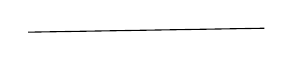
\begin{tikzpicture}\draw[line width=0.4pt] (0,0) -- (3,0.05);\end{tikzpicture}}

De ces cogitations essentiellement géométriques, je ne saurais à l'heure actuelle tirer un programme précis de développement de structures algébriques adéquates pour les exprimer. Je me bornerai à quelques remarques en marge.

\deleted{\unsure{a)|$\alpha$)}} Depuis longtemps j'ai été \unsure{intrigu-|intrigué} par l'idée d'une ``linéarisation'' d'un type d'homotopie (ordinaire), i.e. la question du type: Si $X$ est un type d'homotopie, combien d'information cohomologique du type: cohomologie de $X$ à coefficients variables $M$ (constant%
% A compact nontext point below the first constant, near (818,1807); origin uncertain.
\raisebox{-0.6ex}[0pt][0pt]{\parbox{0pt}{\figure{\begin{tikzpicture}[overlay,x=1mm,y=1mm]\fill (-5,0) circle (0.09);\end{tikzpicture}}}} ou constant tordus),
% Short detached upright mark above the beginning of structure, near (271,1838); origin uncertain.
\raisebox{2ex}[0pt][0pt]{\parbox{0pt}{\figure{\begin{tikzpicture}[overlay,x=1mm,y=1mm]\draw[line width=0.4pt] (1.4,0.2) -- (1.45,-0.2);\end{tikzpicture}}}}structure multiplicative $\deleted{\unsure{=|+}}H^i(X,M)\times H^j(X,N)\unsure{-|\to}H^{i\unsure{\cdot|+}j}(X,M\otimes N)$, plus éventuellement d'autres opérations cohomologiques -- est-il%
% Separate bent stroke at the right of this manuscript line, around (1619,2077); no lexical role assigned.
\raisebox{0.4ex}[0pt][0pt]{\parbox{0pt}{\figure{\begin{tikzpicture}[overlay,x=1mm,y=1mm]\draw[line width=0.4pt] (8,0.3) -- (8.1,0) -- (8.35,-0.2);\end{tikzpicture}}}} nécessaire d'avoir pour \unsure{réconstituer|rêconstituer} le type d'homotopie entièrement \deleted{?}? (disons,
